\subsubsection{Gestione generale delle richieste}
Segue un elenco ordinato dei \textit{middleware\ped{G}} utilizzati, l'ordine di elaborazione della richiesta è determinante poiché ciascuno costituisce un \textit{handler\ped{G}} del \textit{design pattern\ped{G}} \textit{Chain of responability\ped{G}} ed ha la facoltà di interrompere la catena del chiamante:

\begin{itemize}
	\item \texttt{express.compress()}: \textit{middleware\ped{G}} per comprimere ccon il formato \texttt{gzip} le comunicazioni;
	\item \texttt{express.logger()}: \textit{middleware\ped{G}} utilizzato per registrare un log delle richieste, utile per fare il \textit{debugging\ped{G}} dell'applicazione;
	\item \texttt{express.json()}: \textit{middleware\ped{G}} che estrae dalla richiesta i parametri che sono nel formato \textit{JSON\ped{G}};
	\item \texttt{express.urlencoded()}: \textit{middleware\ped{G}} che estrae dalla richiesta i parametri di tipo \\ \texttt{www-form-encoded}, questi possono essere inviati ad esempio conun richiesta POST;
	\item \texttt{express.methodOverride()}: \textit{middleware\ped{G}} utilizzato per permettere anche ai vecchi \\ \textit{browser\ped{G}} di avere un modo per fare richieste PUT e DELETE;
	\item \texttt{express.cookieParser()}: \textit{middleware\ped{G}} che analizza i \textit{cookie\ped{G}};
	\item \texttt{express.cookieSession()}: \textit{middleware\ped{G}} che permette di memorizzare i record della sessione utente per mantenerne lo stato di login;
	\item \texttt{express.ruote()}: \textit{middleware\ped{G}} che permette di configurare un singolo \textit{ruote\ped{G}}, nell'organizzazione interna \texttt{QuizziPedia::Back-End::App::Routers} ogni modulo router contiene i routers logicamente correlati;
	\item \texttt{AuthenticationController}: \textit{middleware\ped{G}} scritto dai \textit{progettisti} per gestire l'autenticazione. Utilizza nello specifico:
			\begin{itemize}
				\item \texttt{passport.authenticate()}.
			\end{itemize}
	\item \texttt{NotFoundHandler}: \textit{middleware\ped{G}} scritto dai \textit{progettisti} per gestire le richieste che non vengono gestite da nessun \textit{controller\ped{G}} (errore \textit{client\ped{G}} 404);
	\item \texttt{ErrorHandler}: \textit{middleware\ped{G}} scritto dai \textit{progettisti} per gestire gli errori sollevati da altri \textit{middleware\ped{G}} (errore \textit{server\ped{G}} 500).
\end{itemize}

Nel seguente \textit{diagramma di sequenza} viene rappresentata una generica richiesta del \textit{client\ped{G}} al \textit{server\ped{G}}. Le classi ed il loro comportamento sono stati progettati in funzione del \textit{design pattern\ped{G}} \textit{Chain of responsability\ped{G}} che viene utilizzato internamente da \textit{express\ped{G}} (§A.3.1).

\label{Gestione richiesta generica}
\begin{figure}[ht]
	\centering
	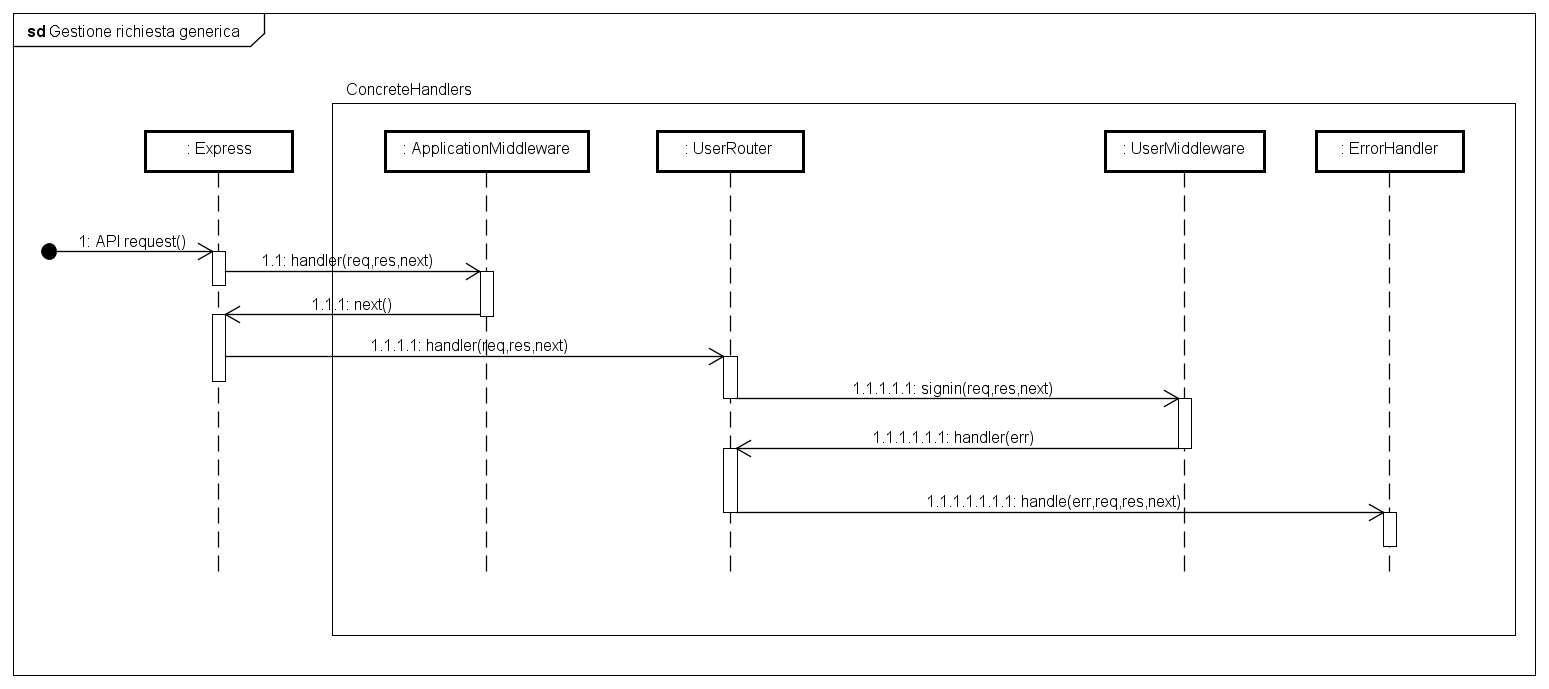
\includegraphics[scale=0.39]{UML/DiagrammiDiSequenza/Back-end/GestioneRichiestaGenerica.png}
	\caption{Gestione di una richiesta dal client}
\end{figure}
\FloatBarrier
